% !TeX root = ../main.tex
\section{面积约束下的算力配比设计空间探索}
\label{sec:workload}

本节以四种 DP 的面积、原生点积长度和活动功耗为输入，在统一整核面积预算下，分别求解混合精度负载的延迟与计算能耗最优配比。分析对象是计算资源充分利用时的 GEMM 服务时间；带宽、边界利用率和调度损失尚未计入，因此结果用于刻画配比的计算侧收益。

\subsection{从单 DP 成本到整核部署}
\label{sec:k4_area}

每个 AI 核心采用 $m=n=16$ 的 DP 阵列。参考计算单元面积构成研究~\cite{luo2024hifloat8area}及公开核心数量~\cite{huawei950}，取基准阵列面积占比 $\alpha=0.30$、基准核心数 $N_0=36$，构造等效预算；该预算不代表实际芯片面积。

令配比 $j$ 的单 DP 面积为 $a_j$，阵列面积为 $A_{T,j}=mn a_j$，下标 0 表示 $1:2:4$。基准整核面积、固定外围面积和总预算为
\begin{equation}
A_{C,0}=\frac{A_{T,0}}{\alpha},\quad
A_O=A_{C,0}-A_{T,0},\quad
A_{\mathrm{bud}}=N_0A_{C,0}.
\label{eq:k4_area_definition}
\end{equation}
保持每核外围面积 $A_O$ 不变，在 $A_{\mathrm{bud}}=496.59$\,mm$^2$ 内部署的完整核心数为
\begin{equation}
n_j=\left\lfloor\frac{A_{\mathrm{bud}}}{A_O+A_{T,j}}\right\rfloor.
\label{eq:core_area_budget}
\end{equation}
以 $p\in\{H,Q,E\}$ 表示精度，$K_{j,p}$ 为单 DP 的原生点积长度，$p_{j,p}$ 为第~\ref{sec:evaluation} 节测得的模式功耗。在 $f=1$\,GHz 下，总峰值算力与 DP 活动功耗为
\begin{equation}
C_{j,p}=2fmn n_jK_{j,p},\qquad
P_{j,p}=mn n_jp_{j,p}.
\label{eq:k4_capacity_power}
\end{equation}

\begin{table}[t]
\centering
\caption{面积预算下的部署结果。$A_C$：整核面积（mm$^2$）；$C$：峰值算力（TFLOP/s）；$P$：仅 DP 的活动功耗（W）。}
\label{tab:k4_absolute}
\begingroup\footnotesize\setlength{\tabcolsep}{3pt}
% Generated by scripts/reproduce.py.
\begin{tabular*}{\linewidth}{@{\extracolsep{\fill}}lrrcc@{}}\toprule
Ratio & $A_C$ & $n$ & $C_H/C_Q/C_E$ & $P_H/P_Q/P_E$ \\\midrule
$1:2:4$ & 11.266 & 36 & 415.8/831.7/1663.3 & 233.1/232.5/223.3 \\
$1:2:6$ & 12.053 & 33 & 381.2/762.3/2287.0 & 219.3/218.7/260.3 \\
$1:2:8$ & 12.567 & 32 & 369.6/739.2/2957.0 & 210.8/210.1/297.3 \\
$1:4:8$ & 13.615 & 29 & 335.0/1339.9/2679.8 & 192.7/320.1/301.3 \\
\bottomrule\end{tabular*}

\endgroup
\end{table}

四种配比分别可部署 36、34、32、29 个核心（表~\ref{tab:k4_absolute}）。$1:2:8$ 与 $1:4:8$ 的单 DP E 吞吐相同，但前者可部署更多核心，获得更高 E 总算力；后者则以部署密度下降换取更高 Q 总算力。单 DP 的吞吐优势因此不能直接等同于固定面积下的系统收益。

\subsection{混合精度负载与优势区域}
\label{sec:k4_simplex}

令 $F_p$ 为精度 $p$ 的有效 GEMM 工作量，$F=\sum_pF_p$，$x_p=F_p/F$，且 $\sum_p x_p=1$。假设各精度阶段顺序执行并充分利用全部核心，计算延迟与 DP 能耗分别为
\begin{align}
T_j&=F\sum_p\frac{x_p}{C_{j,p}},
\label{eq:k4_time}\\
\mathcal E_j&=F\sum_p x_p\frac{P_{j,p}}{C_{j,p}}.
\label{eq:k4_energy}
\end{align}
面积预算覆盖整核，而能耗只包含 DP 计算部分，未加入外围、存储和数据传输。本文分别最小化 $T_j$ 与 $\mathcal E_j$，不将两者合并为单一评分。

在 H/Q/E 三角域内，以 1 个百分点的间隔扫描 5,151 种工作量组成。固定 $F$ 时，两项目标均为 $\boldsymbol x$ 的线性函数，任意两种配比的等成本条件给出直线边界。图~\ref{fig:k4_time_prefill} 标注最优区域的几何面积占比，不代表应用出现概率。

\begin{figure}[t]
\centering
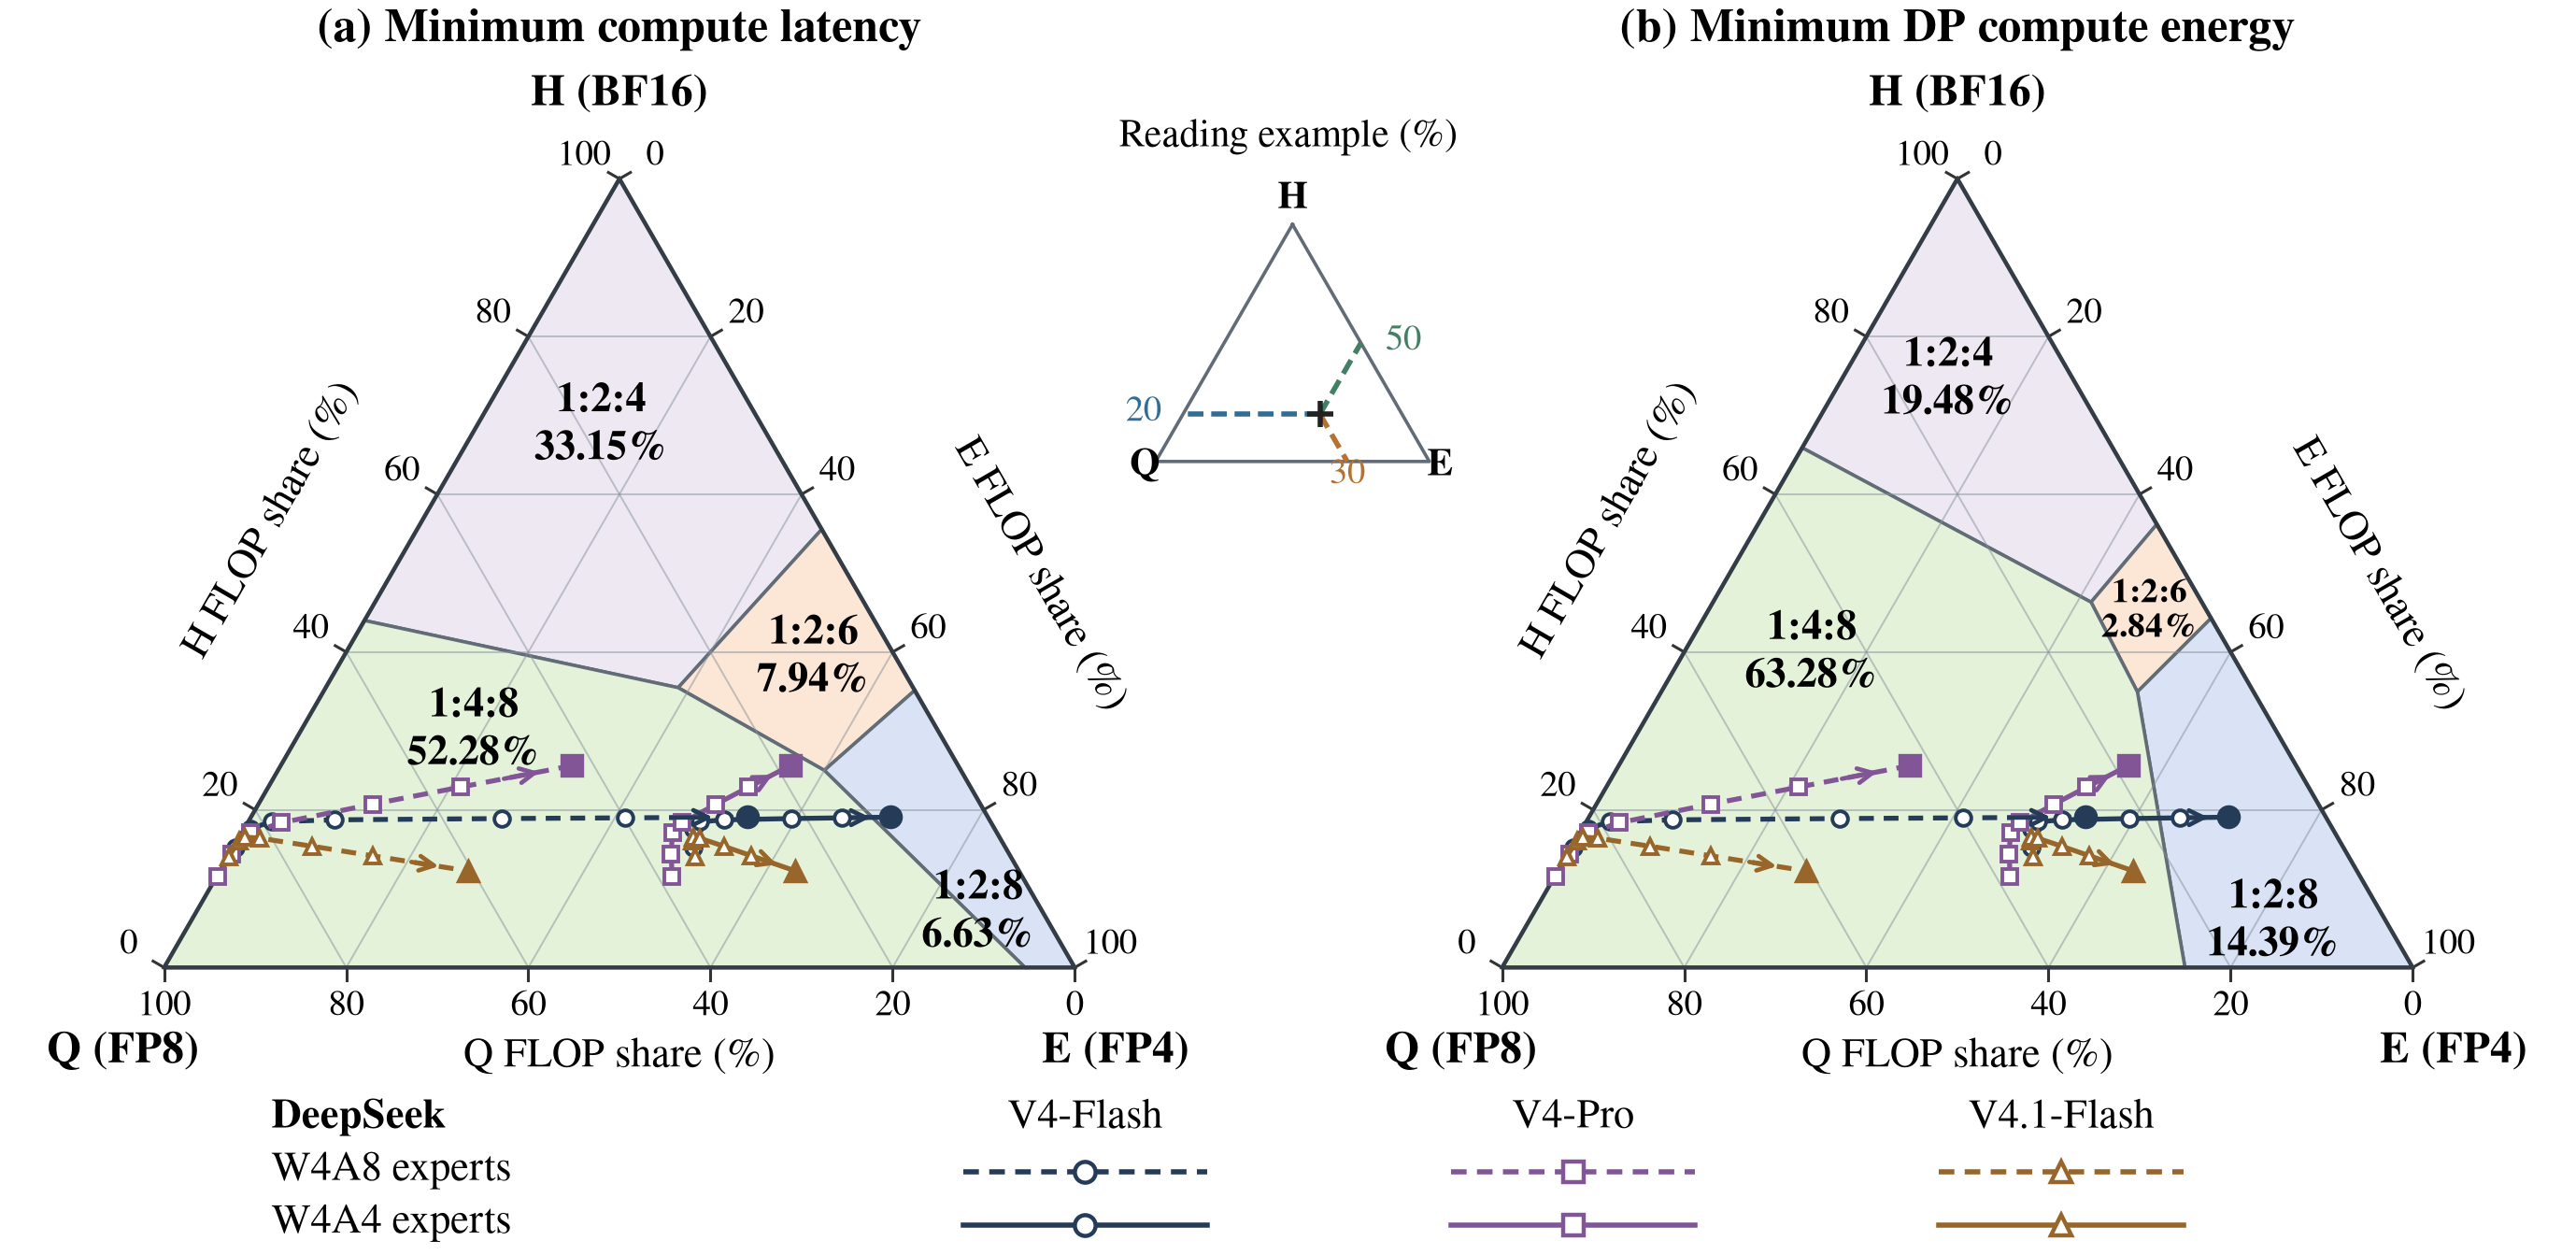
\includegraphics[width=\columnwidth]{k4_n12_prefill_comparison.png}
\caption{等面积下的配比选择：(a) 计算延迟；(b) DP 计算能耗。区域标注为最优配比及其几何占比，小图示例为 H/Q/E=20\%/30\%/50\%。轨迹由 DeepSeek 模型结构导出，虚线为专家 W4A8，实线为专家 W4A4 迁移场景，其余计算不变。箭头依次对应 1K、4K、16K、64K、256K、512K、1M 上下文，实心标记为 1M。NVFP4 能耗使用 MXFP4 功耗代理。}
\label{fig:k4_time_prefill}
\end{figure}

H、E、Q 密集区域分别倾向于 $1:2:4$、$1:2:8$ 和 $1:4:8$；$1:2:6$ 在 H/E 混合且 Q 较少时，以较小面积增量平衡 E 加速与 H 吞吐损失。延迟由各阶段的 $F_p/C_{j,p}$ 决定。单位 FLOP 能耗为 $P_{j,p}/C_{j,p}=p_{j,p}/(2fK_{j,p})$，在当前模型中与核心数抵消，因此延迟与能耗的优势区域不完全重合。

\textbf{观察二：面积约束改变了峰值配比的收益顺序。} 增配低精度通路会减少核心数量，H 阶段无法从单核增配中获益；只有被加速阶段节省的时间足以补偿其余阶段的吞吐损失时，增配才降低总延迟。

\subsection{模型工作量与执行精度映射}
\label{sec:workload_extraction}

工作量统计以 GEMM 算子而非参数存储量为单位。依据固定模型配置和计算规则，确定各投影、注意力及专家算子的 $M,N,K$ 和调用次数，再按 $2MNK$ 汇总。MoE 只计实际激活专家；稀疏或压缩注意力按其有效计算结构统计。每个算子依据权重、激活及执行方式归入 H/Q/E，其他精度单独保留，不强行映射。例如，专家权重虽以 4 位存储，W4A8 执行仍归入 Q；仅当该算子采用 W4A4 执行时才归入 E。

当前采用固定配置与模型特定规则进行可复算的静态分析，后续将结合自动化算子提取与执行轨迹，核验实际内核精度并扩展模型覆盖。
% 后续实验：补入固定版本的 DeepSeek-V3.2；可选完整 DeepSeek-R1。
% 两个实际专家量化版本须分别核验 checkpoint、执行后端与算子覆盖，
% 不能将下述 W4A4 迁移场景直接称为两个已验证量化模型。

\subsection{DeepSeek 负载与低精度迁移}
\label{sec:k4_prefill}

依据官方配置~\cite{deepseekv4,deepseekv4flashsource,deepseekv4prosource,deepseekv41source}，统计 V4-Flash、V4-Pro、V4.1-Flash 在 batch=1、1K--1M 七种上下文下的冷启动 prefill，纳入稀疏/压缩注意力以及 V4.1 的 CED 与索引复用。BF16 注意力与分组输出投影归入 H，W4A8 专家计算和 FP8 投影归入 Q，MXFP4 索引点积归入 E。另构造仅将路由专家改为 NVFP4 W4A4 的迁移场景，其余计算保持不变。两组映射各含 21 个负载点，H/Q/E 覆盖其 GEMM 工作量的 97.11\%--99.37\%；图中的占比仅在这三类内归一化。

全部 W4A8 采样点均以 $1:4:8$ 的计算延迟和 DP 能耗最低。专家迁移至 W4A4 后，V4-Flash 在 512K 的能耗最优配比、1M 的延迟最优配比转为 $1:2:8$，另两模型至 1M 仍选择 $1:4:8$。在 V4-Flash 的 1M 点，$1:2:8$ 相对 $1:4:8$ 的延迟与估计能耗优势仅为 1.45\% 和 2.03\%，说明该点靠近配比边界，不宜据此推断普遍优势。

可进一步用受控迁移描述未来需求：设现有 Q 工作量中有比例 $\lambda$ 转为 E，算子形状与总工作量保持不变，则
\begin{equation}
\boldsymbol x(\lambda)=
\bigl(x_H,(1-\lambda)x_Q,x_E+\lambda x_Q\bigr),\quad 0\le\lambda\le1.
\label{eq:precision_migration}
\end{equation}
将其代入式~\eqref{eq:k4_time} 和式~\eqref{eq:k4_energy} 可分别求得延迟、能耗的配比切换条件。该路径用于隔离执行精度变化的影响，不代表量化后的模型精度已得到验证。

\textbf{观察三：当前与未来的较优配比取决于执行精度迁移。} 采样的 DeepSeek W4A8 结构保留较多 Q 工作量，使 $1:4:8$ 受益；若更多 Q 计算能够转为 E，$1:2:8$ 的部署密度和 E 总算力优势将更有价值。实际切换点同时取决于残留 H/Q 工作量，不能仅凭采用 FP4 权重判断。

模型采用统一 Qwen 活动功耗代理 DeepSeek，并以 MXFP4 代理 NVFP4，未计入格式转换、供数开销及外围面积增长。完整推理收益仍需通过执行轨迹、带宽约束与跨负载功耗校准验证。
